\begin{figure}[!h]
\centering
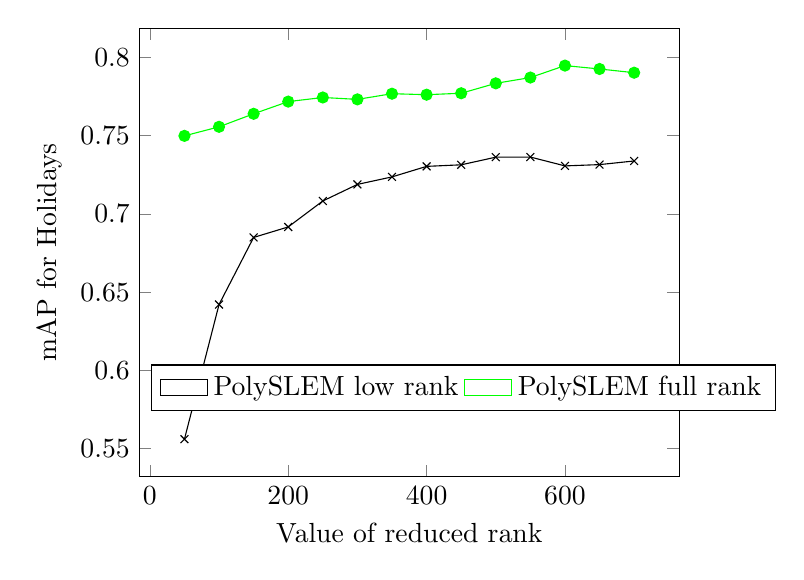
\begin{tikzpicture}
	\begin{axis}[
		xlabel=Value of reduced rank,
		ylabel=mAP for Holidays,
		legend style={
			area legend,
			at={(0.6,0.25)},
			anchor=north,
			legend columns=-1}]
%%Poly SLEM
    \addplot[mark=x, black] coordinates{
         ( 50, 0.5560)
         (100, 0.6421)
         (150, 0.6850)
         (200, 0.6917)
         (250, 0.7083)
         (300, 0.7189)
         (350, 0.7237)
         (400, 0.73043)
         (450, 0.73143)
         (500, 0.73631)
         (550, 0.73639)
         (600, 0.73073)
         (650, 0.73156)
         (700, 0.73388)
    };
    \addlegendentry{PolySLEM low rank}
    \addplot[mark=*, green] coordinates{
        (  50, 0.74994)
        ( 100, 0.75572)
        ( 150, 0.76405)
        ( 200, 0.77184)
       (  250, 0.77447)
         (300, 0.77327)
         (350, 0.77689)
         (400, 0.77626)
         (450, 0.77718)
         (500, 0.78352)
         (550, 0.78723)
         (600, 0.79487)
         (650, 0.79270)
         (700, 0.79032)
    };
    \addlegendentry{PolySLEM full rank}
	\end{axis}
\end{tikzpicture}
\caption{mAP for Holidays using SPoC features. We perform a low-rank decomposition of a $100000\times 100000$ kernel matrix for the low rank curve, whereas we use a full rank decomposition with }
\end{figure}

